\documentclass[a4paper,12pt]{article}
\usepackage[utf8]{inputenc}
\usepackage[polish]{babel}
\let\lll\undefined % do babelu, avoiding conflict
\usepackage{polski}
\selectlanguage{polish}
\usepackage[T1]{fontenc}
\frenchspacing
\usepackage{indentfirst}
\usepackage{multicol} %https://www.sharelatex.com/learn/Multiple_columns
\usepackage{float} % option locking floats: [H]


\usepackage{amssymb}
\usepackage{amsmath}
\usepackage{amsfonts}
 
\usepackage[pdftex,dvipsnames]{xcolor} %red, green, blue, yellow, cyan, magenta, black, white
%polskie tabelki
\usepackage[nottoc]{tocbibind}

% Kropki w liczebnikach porzadkowych
\usepackage{titlesec}
\titlelabel{\thetitle.\quad}


\setlength{\parskip}{0.3\baselineskip}%
% \setlength{\parindent}{0pt}%

%polskie przypisy
\usepackage{caption}
\captionsetup{labelsep=period}
\captionsetup{font=small,labelfont=bf,labelsep=period,justification=centering}
\addto\captionspolish{\renewcommand{\figurename}{Rys.}}
\addto\captionspolish{\renewcommand{\tablename}{Tab.}}
\addto\captionspolish{\renewcommand{\seename}{zob.}}

\usepackage{geometry}
 \geometry{
 a4paper,
 %total={170mm,247mm}, % 170 257 20 20
 left=20mm,
 right=20mm,
 top=20mm,
 bottom=25mm,
 }   
   


\usepackage{listings}
\definecolor{mygreen}{RGB}{28,172,0} % color values Red, Green, Blue
\definecolor{mylilas}{RGB}{170,55,241}
% \newcounter{listing}
% \newenvironment{listing}[1][]{
% \refstepcounter{listing}\par\medskip \textbf{Kod~\thelisting. #1} \rmfamily}{\medskip}

\lstset{language=Matlab,%
    %basicstyle=\color{red},
    breaklines=true,%
    morekeywords={matlab2tikz},
    keywordstyle=\color{blue},%
    morekeywords=[2]{1}, keywordstyle=[2]{\color{black}},
    identifierstyle=\color{black},%
    stringstyle=\color{mylilas},
    commentstyle=\color{mygreen},%
    showstringspaces=false,%without this there will be a symbol in the places where there is a space
    numbers=left,%
    numberstyle={\tiny \color{black}},% size of the numbers
    numbersep=9pt, % this defines how far the numbers are from the text
    emph=[1]{for,end,break},emphstyle=[1]\color{red}, %some words to emphasise
    %emph=[2]{word1,word2}, emphstyle=[2]{style},    
    basicstyle=\small\ttfamily,
    frame=single,
    float
}


\usepackage{svg}
%SVG for the first time using inkscape: for i in *.svg; do inkscape -D -z --file=$i  --export-pdf="${i%.*}.pdf" --export-latex .; done




\usepackage{xargs}                      % Use more than one optional parameter in a new commands
%
\usepackage[colorinlistoftodos,prependcaption,textsize=tiny]{todonotes}
\newcommandx{\unsure}[2][1=]{\todo[linecolor=red,backgroundcolor=red!25,bordercolor=red,#1]{#2}}
\newcommandx{\change}[2][1=]{\todo[linecolor=blue,backgroundcolor=blue!25,bordercolor=blue,#1]{#2}}
% \newcommandx{\info}[2][1=]{\todo[linecolor=OliveGreen,backgroundcolor=OliveGreen!25,bordercolor=OliveGreen,#1]{#2}}
% \newcommandx{\improvement}[2][1=]{\todo[linecolor=Plum,backgroundcolor=Plum!25,bordercolor=Plum,#1]{#2}}
% \newcommandx{\thiswillnotshow}[2][1=]{\todo[disable,#1]{#2}}

% \missingfigure[figwidth=6cm]{Testing a long text string}


\usepackage[section]{placeins} %\FloatBarrier
% \usepackage{hyperref}
   
\usepackage{fancyhdr}
\setlength{\headheight}{38pt}
\pagestyle{fancy}

\lhead{Sprawozdanie z grantu rektorskiego koła SKIK 2016}     \rhead{\today\quad\includesvg[width=1.5cm]{logo_skik}}
\lfoot{}            \cfoot{}        \rfoot{strona \thepage/\pageref{ENDOFDOC}}

\title{Projekt przedmiotu Sieci Neuronowe i Neurokomputery wydziału EiTI Politechniki Warszawskiej}
\author{Artur Dobrogowski}



\begin{document}


\begin{titlepage}
    \centering
    \includesvg[width=0.3\textwidth]{logo_pw}\par\vspace{1cm}
    {\scshape\Large Politechnika Warszawska\\Wydział Elektroniki i Technik Informacyjnych\\Instytut Radioelektroniki i Technik Multimedialnych \par}
    \vspace{1cm}
    {\huge\scshape\bfseries Sprawozdanie\\\par}
    {\scshape\Large z pracy naukowo-badawczej własnej\\ finansowanej z grantu rektorskiego za rok 2016\\\par}
%     {\Large Umowa numer XXX Y/????/????\\\par}
    \vspace{1cm}
    {\Large\bfseries System pomiarowy na pokładzie kapsuły balonu stratosferycznego\\\par}
    \vspace{1cm}
    {\Large\itshape Studenckie koło inżynierii kosmicznej\par}
    \vfill
    Wykonawcy: \par
    {\small
    \begin{multicols}{3}

    \par Artur \textsc{Dobrogowski} 
    \par Michał \textsc{Kocon}
    \par Herbert \textsc{Namirski}
    \par Mateusz \textsc{Chomiczewski}
    \par Maciej \textsc{Trębiński}
    \par Kamil \textsc{Lucyszyn}
    \end{multicols}
}
    Kierownik pracy:\par
    dr inż. Krzysztof \textsc{Kurek}

    \vfill

% Bottom of the page
    {\large \today\par}
\end{titlepage}

\tableofcontents

\section{Wprowadzenie}
% ** o balonach
Balon stratosferyczny pozwala na wyniesienie podczepionego pod nim ładunku na wysokość około 35 km nad poziom morza, co umożliwia realizację różnych pomiarów związanych z dolnymi warstwami atmosfery. Jednocześnie panujące na wysokości kilkudziesięciu km nad ziemią  niskie ciśnienie i niska temperatura pozwalają na test pracy wynoszonych układów w tak niekorzystnych warunkach. Realizacja misji balonowej może być więc prostym i tanim sposobem na sprawdzenie działania opracowanych układów w warunkach zbliżonych do środowiska przestrzeni kosmicznej.
Stratosferyczne misje balonowe są coraz częściej organizowane w Polsce, zarówno przez studentów np. ze Studenckiego Koła Astronautycznego PW, jak  również przez różne stowarzyszenia zrzeszające entuzjastów balonów i radioamatorów.
Również SKIK, w swojej dotychczasowej działalności zrealizował kilka misji balonowych.
\subsection{Cel projektu}
Celem projektu jest zaprojektowanie i skonstruowanie platformy do misji balonowych i zbierania danych z górnych partii atmosfery. Opracowanie systemu pomiarowego w misji balonowej stanowi pewne odwzorowanie problemów z jakimi trzeba się zmierzyć podczas projektowania satelity, ponieważ w trakcie misji nie ma możliwości na poprawki ani usuwanie awarii. Jednym z najważniejszych aspektów jest komunikacja radiowa. Kluczowe jest śledzenie parametrów lotu i warunków panujących na zewnątrz układu, aby wiedzieć czy sprzęt prawidłowo funkcjonuje. W przypadku satelitów, po ukończeniu swojego zadania urządzenia ulegają zniszczeniu przy powrocie do atmosfery, natomiast w misji balonowej ważne jest odnalezienie urządzenia, odzyskanie danych zapisanych na dysku i zapewnienie bezpiecznego powrotu na ziemię.

Zadaniem systemu pokładowego kapsuły jest akwizycja danych w profilu wysokości oraz ich transmisja. Dane uzyskane z misji balonowych są nie do uzyskania w inny sposób, ponieważ samoloty nie wznoszą się tak wysoko, a satelity są w stanie dokonywać tylko pomiarów pośrednich.

\subsection{Czujniki}
Projektowany system zostanie wyposażony w zestaw czujników, mierzących poziom dwutlenku węgla i wilgotności. Pomiar tych gazów jest istotny ze względu na modelowanie pogody jak i klimatu.

Umożliwi to porównanie wyników, uzyskanych podczas planowanej misji balonowej z danymi z lat poprzednich i oszacowanie jak ludzka działalność przyczyniła się do zmian składu atmosfery. Poza tym zbieranie i publikowanie takich danych przez niezależne instytucje da lepszy wgląd w modelowanie klimatu i pomoże przyspieszyć akcję zapobiegające zmianom klimatycznym.

Platforma balonowa będzie się składać z:
\begin{itemize}
 \item komputera pokładowego Raspberry PI zero
 \item kamery nagrywającej lot do celów promowania koła
 \item moduł z czujnikiem do pomiaru stężenia dwutlenku węgla
 \item czujnik wilgotności
 \item czujnik ciśnienia
 \item czujnikami temperatury wewnątrz i na zewnątrz kapsuły
 \item modułu komunikacyjnego 433 MHz
 \item moduł zasilania
 \item modułu GPS
\end{itemize}

Oprócz tego w platformie będą umieszczone niezależne układy lokalizacyjne:
\begin{itemize}
 \item układ APRS będący tematem pracy magisterskiej absolwenta i honorowego członka koła: Mateusza Walczyka
 \item lokalizator GPS-GSM z kartą SIM
\end{itemize}

 
%opis ogólny co mialo byc zrobione i po co
% misje balonowe, parametry mierzone, co jest istotne, w funkcji wysokosci
\section{Opracowanie projektu systemu pomiaru zanieczyszczeń i innych czujników}

\begin{figure}[htpb]
\centering
\includegraphics[width = 0.8\textwidth]{ukl_pom.png}
\captionof{figure}{Schemat połączeń dla płytki pod układ z przetwornikiem analogowo-cyfrowym ADuCM360}
 \label{schem}
\end{figure}


\subsection{Uzasadnienie wyboru zestawu czujników}

\begin{itemize}
\item \textbf{pomiar wysokości}: wysokość balonu jest ważnym parametrem do precyzyjnego zmierzenia , ponieważ chcemy zbadać zmienność parametrów w funkcji wysokości. Wynik wysokości ustalamy na podstawie uśredniania danych szacowanych z różnych źródeł:
\begin{itemize}
 \item zakładając wznoszenie ruchem jednostajnym (z ewentualnymi korektami z akcelerometru), oraz znając wagę gondoli i wyporność balonu jest ustalana na podstawie obliczeń z pomiarem czasu zegarem pokładowym
 \item znając przybliżoną z pomiarów innych osób dostępnych w internecie - zależność ciśnienia w funkcji wysokości - jest to wartość szacowana ponieważ jest zmienna np z warunkami pogody.
\item z danych GPS% coś jeszcze?
\end{itemize}
\item \textbf{pomiar temperatury}: Wewnątrz gondoli jest nam potrzebny zarówno ze względu na wprowadzenie korekty na pomiar innych czujników stwierdzenie czy układy zachowują się poprawnie i mieszczą się w sprecyzowanym przez producenta przedziale temperaturowym. Na zewnątrz gondoli jest daną której trend (zbierane wielokrotnie przez długi okres czasu)  jest parametrem modelu klimatu. Nasz pomiar jest tylko orientacyjny i porównamy jego poprawność z danymi zbieranymi przez profesjonalistów w tej dziedzinie - instytut meteorologii.
\item \textbf{wilgotność}: podobnie jak temperatura, wartość chwilowa tego parametru świadczy jedynie o obecnej pogodzie, a nie o stanie klimatu. Dopiero długookresowe pomiary średnich poziomów tego parametru są danymi do modelowania klimatu. Również w tym przypadku naszym celem jest porównanie tego pomiaru z danymi pobieranymi przez instytut meteorologii i dostarczenie kolejnego punktu pomiarowego do obrazu. W dodatku wartość tego parametru może wpływać na odczyt pozostałych czujników, więc jego znajomość pozwoli nam na ewentualne korekty pomiarów.
\item \textbf{położenie}: oczywiście, musimy znać położenie naszego punktu pomiarowego jak i gondoli, żeby ją później odzyskać. Na podstawie zmienności położenia w czasie ustalamy prędkość wiatru jaki panuje na danej wysokości.
\item \textbf{orientacja}: bardziej dla celów poznawczych dla przyszłych misji chcemy poznać stabilność gondoli względem słońca i zmierzyć poziom huśtania i obracania. Przydadzą nam się dane, żeby stwierdzić jakiej stabilizacji potrzebowały by układy optyczne na gondoli takie jak spektroskop (analizator widma) czy ogniwa fotowoltaiczne.
\end{itemize}

Czujniki jakie wybraliśmy pozwalają na zmierzenie powyższych parametrów w zadowalającej dokładności, oraz były finansowo atrakcyjne. W dodatku przy wyborze braliśmy pod uwagę jak najniższą dopuszczalną temperaturę czujników, jak i kompatybilność interfejsów i poziomów zasilania i logiki dla układów cyfrowych.

\subsection{Wybór czujników do systemu pomiaru zanieczyszczeń}

Przez pomiar zanieczyszczeń rozumiemy zanieczyszczanie atmosfery w skali globalnej przez działalność ludzką. Pod tę kategorię mogą przypadać różne gazy: związki azotu, siarki, czy węglowodory, a także pyły i areozole, radioizotopy. Niektóre gazy spodziewane w atmosferze (takie jak np. ozon) są pożądane w pewnych ilościach, ale traktowane jako zanieczyszczenie jeśli są znalezione poza swoją strefą występowania. Ozon przy powierzchni ziemi powstaje przy niektórych gałęziach przemysłu lub wyładowaniach elektrycznych przy burzy i jest traktowany jako substancja szkodząca - czyli zanieczyszczenie.

Naszą uwagę skupiliśmy na ogólnej działalności przemysłu która przyczynia się do ocieplania klimatu. Związane z tym związki to przede wszystkim bezpośrednio: (dwu)tlenek węgla ($CO_2$), metan ($CH_4$), jak i (pośrednio) para wodna ($H_2O$). Na początku mieliśmy plan mierzyć wszystkie trzy i do tego jeszcze ozon, ale stanęło na pomiarze dwutlenku węgla i pary wodnej. Zrezygnowaliśmy z ozonu i metanu ze względu na ograniczone finanse. 

Aby precyzyjnie mierzyć stężenie takich gazów, należy ustandaryzować warunki do pomiaru: najlepiej stałe ciśnienie i temperatura. Nad temperaturą nie możemy wiele poradzić, ponieważ powietrze które będziemy próbkować jest bardzo zimne, ale możemy sprężać i rozprężać powietrze w zamkniętym cylindrze. Ponieważ jednak jesteśmy na wydziale elektroniki i technik informacyjnych, chcieliśmy pierwszą misję po reaktywacji koła utrzymać możliwie prostą i ograniczyć rozwiązania w kwestiach mechanicznych. Odłożyliśmy realizację tego rozwiązania na przyszłą misję. W ramach testów taniego cylindra do sprężania, podczepimy pod gondolą zakręconą butelkę PET aby sprawdzić czy wytrzyma różnicę ciśnień.

Teorytycznie oba efekty - wpływ ciśnienia i temperatury można skorygować, ale problem pojawia się jeżeli przez te efekty wartość mierzona spada poniżej rozdzielczości czujnika.

Istnieją dwie główne realizacje takich czujników gazowych: działających na zasadzie elektrolizy, lub optyczne - na zasadzie absorpcji. Te drugie są zdecydowanie lepsze do wykrywania małych stężeń jakie będą mierzone, więc zdecydowaliśmy się na czujniki optyczne.

\subsection{Wybór modułu komunikacyjnego}

Moduł HM-TRLR-S został przez nas wybrany ze względu na pracę w paśmie radio-amatorskim 433MHz oraz dużą czułość odbiornika przy wykorzystaniu modulacji LoRa. Pozwala to na uzyskanie dużych zasięgów nadajnika, które będą potrzebne do uzyskania stałej łączności aparatury pomiarowej ze stanowiskiem odbiorczym znajdującym się przy powierzchni ziemi.

Dodatkowym atutem modułu jest jego niska waga oraz kompaktowe rozmiary, co pozwoliło na odciążenie gondoli balonu. Niska częstotliwość fali nośnej pozwala na mniej stratną propagację w atmosferze.

Wybraliśmy też ten moduł ze względu na szacowaną odległość odbioru dla widoczności w wolnej przestrzeni (jakiej układ na balonie jest dobrym przybliżeniem). Przy nadawaniu z mocą 0.1W, moc odbierana: $P_{R[dBmW]} = P_{T[dBmW]} + G_{T[dBi]} + G_{R[dBi]} -L_{FS[dB]}$, gdzie tłumienie w wolnej przestrzeni $L_{FS} = \left ( \frac{4\pi R}{\lambda}\right )^2$.

Modulacja LoRa w tym nadajniku pozwala na dużą czułość odbiornika na poziomie -139dBm. Oznacza to, że z dobrym marginesem powinniśmy odebrać sygnał z balonu na wysokości 35 km w promieniu 40 km od balonu, ponieważ tłumienie w wolnej przestrzeni wyniesie $L_{FS} \simeq 120 dB$, podczas gdy $P_T = 20 dBmW$, czyli sygnał odbierany będzie na poziomie $-100 dBmW$.

\section{Realizacja systemu}

% 3. Opis poszczególnych elementów ze schematu blokowego z rozdziału 2 - schematy ideowe, schematy płytek drukowanych, oprogramowanie pozwalające na podłączenie czujników do Rasberry PI, zasilanie, gondola, spadochron, element odblaskowy zapewniający widoczność na radarze (jeśli nie ma z przykładowych sprawozdaniach, które podesłałem, to powinien być opisany w pracy Mateusza Walczyka, do tego również  można powołać się na jego układ APRS i go opisać, podając odwołanie do jego pracy).


Całość składa się czterech głównych części: balonu, spadochronu, gondoli i odblasku radiowego. W gondoli umieszczono system elektroniczny dbając o izolację termiczną i wystawiając czujniki gazów i temperatury poza gondolę umożliwiając dobry kontakt z mezurandem i wymianę gazów. Reflektor wykonano z folii aluminiowej i tektury w celu zapewnienia dobrej widoczności radarowej balonu przez pojazdy latające i urządzenia nawigacyjne.


System elektroniczny balonu zrealizowano w oparciu o układ Raspberry Pi Zero, które służy jako komputer pokładowy i jest najwyższy w hierarchii modułów, ponieważ odpowiada za gromadzenie danych oraz ich przetwarzanie.

% \begin{figure}[H][htbp!]
% \centering
\begin{figure}[H]
\includegraphics[width = 0.9\textwidth]{schemat.pdf}
\centering\captionof{figure}{Schemat połączeń dla płytki pod układ z przetwornikiem analogowo-cyfrowym ADuCM360}
 \label{schem}
\end{figure}
% \end{figure}


System czujników składa się z między innymi o interfejsie analogowym (barometr i czujnik wilgotności). Pomiar czujników analogowych został zrealizowany na mikrokontrolerze ADuCM360 z 24 bitowym przetwornikiem analogowo-cyfrowym. Dla tych sygnałów było potrzebne wzmocnienie aby w pełni wykorzystać zakres naszego przetwornika i uzyskać najlepszą dokładność. Ponieważ mamy do czynienia z sygnałami wolno-zmiennymi zastosowaliśmy proste układy z wykorzystaniem wzmacniaczy operacyjnych. Komunikacja z komputerem pokładowym została zrealizowana za pomocą protokołu I2C, które zostało wyprowadzone na goldpin zgodny z wyprowadzeniami z raspberry pi zero (P2).  Porty układu zostały wyprowadzone odpowiednio na goldpin - w tym także złącze programujące komunikujące się za pomocą UART - P0.1 i P0.2 w P6, oddzielnie natomiast interfejs programujący SWD - P1. Dodano także filtr zasilania części analogowej i cyfrowej układu zgodnie z dokumentacją ADUCM360/361 (wartośc indukcyjności cewki nie musi być 100mH, jest to wartość domyślna dla programu altium, w układzie wykorzystano 10uH). Dodano także rezonator kwarcowy pozwalający na precyzyjne odmierzanie czasu. W układzie są dwa ``microswitch-e'' - jeden resetujący mikrokontroler (SW1), drugi włączający tryb programowania przez UART (SW2).

Zastosowane oprogramowanie na układzie ADuCM360 mierzy wartości na wejściu układu i przesyła je bezpośrednio do przetworzenia do komputera pokładowego. Układ ADuCM360 pozwala także na poszerzenie ilości dołączonych modułów i układów w przyszłości (posiada kilka portów, które mogą zostać jeszcze wykorzystane jak SPI, UART, DAC, PWM i nie wykorzystane GPIO).


\begin{figure}[H]
\includegraphics[width = 0.5\textwidth]{plytka.jpg}
\centering\captionof{figure}{Zdjęcie wykonanej płytki APRS, wg. pracy Mateusza Walczyka \cite{aprs}}
 \label{plytka}
\end{figure}

Czujniki cyfrowe oraz moduły telekomunikacyjne zostały podłączone bezpośrednio do komputera pokładowego (raspberry pi zero). Odczyt czujnika  MH-Z14A (pomiar CO2) został zrealizowany za pomocą pomiaru czasu wypełnienia okresu sygnału (więcej w dokumentacji czujnika). Moduł Pololu (akcelerometr, barometr, magnetometr i żyroskop) został podłączony za pomocą I2C do komputera pokładowego. Za pomocą 1-wire podłączono termometr DS18S20+ do GPIO. Resztę (GPS) podłączono za pomocą portu UART. W obsłudze modułu GPS wykorzystano dodatkowo gotową bibliotekę tinyGPS++, która ma zaimplementowany protokół NMEA. Obsługę wszystkich portów komputera pokładowego zrealizowano dzięki bibliotece wiringPi, która pozwoliła na bezpośrednie przeniesienie programów z arduino na nasz komputer pokładowy.




Ze względu na konieczność elastyczności w rozmieszczaniu modułów w gondoli, zdecydowaliśmy się nie wykonywać połączeń między modułami na płytce, a łącząc moduły przylutowanymi przewodami, lub przy użyciu zabezpieczonych taśmą wtyczek.


\section{Testowanie i integracja systemu}

\begin{figure}[H]
\includegraphics[width=0.7\textwidth]{arduino_test.png}
\centering\captionof{figure}{Zdjęcie z (prawie) wszystkimi czujnikami i układami do ich przetestowania.}
\end{figure}

Każde urządzenie testowaliśmy niezależnie na platformie arduino, testując czy układ działa w temperaturze pokojowej i około $-10^oC$ które panowało na zewnątrz.

Wyniki były zgodne ze specyfikacjami urządzeń, za wyjątkiem aparatu, który dostaliśmy wadliwy i oczekujemy na rozpatrzenie naszej reklamacji.

Oprócz naszego układu, dostaliśmy wykonany przez mgr. Mateusza Walczyka układ APRS do lokalizacji, który jest układem z niezależnym od naszego zasilaniem i pozycjonowaniem GPS.

W gondoli umieściliśmy również lokalizator GSM do pewniejszego odnalezienia gondoli po powrocie na ziemię. Urządzenie to umożliwia uzyskanie lokalizacji po odpytaniu przy pomocy wiadomości SMS.

\subsection{Testowanie systemu pomiaru zanieczyszczeń}

\begin{figure}[H]
\includegraphics[width=0.5\textwidth]{swieczka_test.png}
\centering\captionof{figure}{Zdjęcie z testowania czujnika CO2.}
\label{swieczka}
\end{figure}

Mamy na uwadze, że parametry które będą mierzone nie będą się zmieniać dynamicznie, ale dla weryfikacji wykonaliśmy test bezwładności pomiaru czujnika dwutlenku węgla. Nasz czujnik operuje w zakresie 0-5000 ppm, a biorąc pod uwagę że w atmosferze jest średnio około 400-700 ppm cząsteczek CO2, nie trzeba wiele aby go nasycić. Dla ustandaryzowania testu wybraliśmy jeden przezroczysty pojemnik widoczny na zdjęciu \ref{swieczka} i zapaliliśmy pod nim świeczkę, której zgaścięcie oznaczało przemianę większości objętości tlenu pod pojemnikiem w procesie spalania na dwutlenek węgla. Stężenie CO2 takiej mieszaniny wielokrotnie przeywższa 5000 ppm. 

\begin{figure}[H]
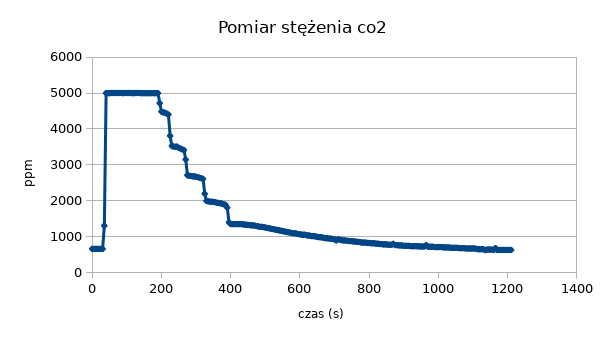
\includegraphics[width=0.7\textwidth]{co2.png}
\centering\captionof{figure}{Testowanie bezwładności czujnika CO2.}
\end{figure}

W stanie równowagi przed pomiarami wartość odczytywana oscylowała wokół 655 ppm. Jest to wartość powyżej średniej globalnej, ale spodziewana. Szczególnie zimą w niewielkim nie klimatyzowanym pomieszczeniu w dużym mieście.

Po wypaleniu świeczki pod przykryciem i odczekaniu paru minut ostrożnie umieściliśmy tam nasz czujnik. Nie umieszczaliśmy czujnika razem z zapaloną świeczką z obawy na zastrzeżoną w dokumentacji wrażliwość czujnika na ciepło i promieniowanie. Na powyższym wykresie widać odpowiedź naszego czujnika. Odpowiedź zobaczyliśmy po upływie około 30 sekund prawie natychmiastowego nasycenia, po czym zdjęliśmy przykrywkę uwalniając zgromadzony gaz i mierzyliśmy czas jaki zajmie powrót do pierwotnego stanu równowagi.



\begin{figure}[H]
\centering
\includegraphics[width=0.7\textwidth]{stanowisko_test.png}
\captionof{figure}{Zdjęcie z stanowiska gdzie odczytywaliśmy pomiary czujnika CO2. Połączenie z RPI było zrealizowane za pośrednictwem routera WiFi}
\end{figure}


\subsection{Integracja systemu}

Ze względu na wybór czujników, poza UART nie mieliśmy konfliktów interfejsów i wszystkie cyfrowe wyjścia danych mogliśmy podłączyć bezpośrednio do komputera pokładowego. Konflikt wielu interfejsów UART rozwiązaliśmy za pośrednictwem układu ADUCM360 tłumacząc wejście UART na $I^2C$, a drugi konflikt - korzystając z alternatywnego wyjścia PWM czujnika. Dla czujników analogowych wykonaliśmy płytkę (wg. schematu z rysunku \ref{schem}) pod układ z precyzyjnym przetwornikiem analogowym ADUCM360, którego wyjścia cyfrowe podłączyliśmy do pinów GPIO komputera pokładowego.

Ze względu na duży pobór mocy niektórych czujników (np. MH-Z14A) został wykorzystany oddzielny stabilizator zasilania LM7805.
Zasilanie jest w postaci czterech równolegle połączonych paczek składających się z szeregowo połączonych dwóch akumulatorów o napięciu nominalnym 3.6-3.7V.

\subsection{Stacja naziemna}

Na stację naziemną składa się komputer z podłączonym odbiornikiem w postaci komputera OrangePi z podłączonym modułem komunikacyjnym w postaci odbiornika z takimi samymi ustawieniami jak nadajnika w gondoli. Do tego została zrealizowana antena kierunkowa. Stacja naziemna ma na celu odbieranie danych nadawanych przez stację w balonie. Będzie zlokalizowana w samochodzie i umożliwi śledzenie ``na żywo'' lokalizacji balonu i umożliwi nam odzyskanie gondoli ze spadochronem po zakończeniu misji.

\section{Realizacja misji balonowej}

W celu zrealizowania misji, oprócz tzw. ładunku jaki ma zostać wyniesiony w stratosferę, trzeba dodatkowych przygotowań. Niezbędne są: 
\begin{itemize}
 \item zakupiony balon, wraz z gazem do napompowania ($H_2$, albo $He$), jak na rys. \ref{balon}.
 \item wykonanie lub kupno spadochronu. Wykonaliśmy własny spadochron pokazany na rys. \ref{spadochron} razem z gondolą
 \item wykonanie kapsuły na układy elektronicznie, zwanej potocznie gondolą
 \item wykonanie reflektora radarowego - w celu zapewnienia dobrej widoczności nawigacji pojazdów latających (takich jak samoloty) posługujących się radarem
 \item uzyskanie okna czasowego i zgody na start Polskiej Agencji Żeglugi Powietrznej PAŻP w danym rejonie 
\end{itemize}

\begin{figure}[H]
\includegraphics[width = 0.7\textwidth]{spadochron.jpg}
\centering\captionof{figure}{Amatorski spadochron wykonany do celów misji, wraz z gondolą w siedzibie SKIK}
\label{spadochron}
\end{figure}

\begin{figure}[H]
\includegraphics[width=0.35\textwidth]{reflektor.jpg}
\centering\captionof{figure}{Reflektor radarowy do podwieszenia pod gondolą.}
\label{reflektor}
\end{figure}

\begin{figure}[H]
\centering
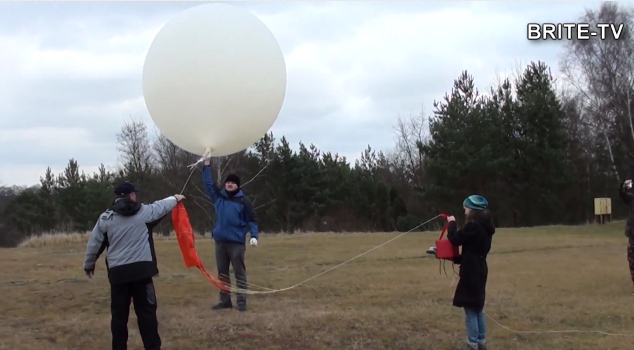
\includegraphics[width=0.6\textwidth]{balon.png}
\captionof{figure}{Zdjęcie balonu gotowego do startu z poprzednich misji}
\label{balon}
\end{figure}

Wszystko wymienione powyżej, za wyjątkiem pozwolenia na start zostało wykonane i przetestowane i jest gotowe do odbycia misji.

Początkowo start misji był zaplanowany na jesień 2016, ale ze względu na około jednomiesięczne przeciągnięcie się prac związanych z wykonaniem i integracją systemu, start misji balonowej musiałby się odbyć na przełomie grudnia i stycznia 2016 r. Chcąc uniknąć realizacji tego zadania w warunkach ujemnych temperatur i dużego zachmurzenia (system zawiera kamerę nagrywającą obraz powierzchni Ziemi w czasie lotu balonu), przyjęto, że wysłanie balonu zostanie przesunięte na okres wiosenny 2017 roku.

Ze startem balonu stratosferycznego z opracowanym systemem na pokładzie związana będzie akcja promująca działalność Koła m.in. poprzez ogłoszenie konkursu dla radioamatorów na odbiór danych APRS wysyłanych z balonu, czy akcja śledzenia lecącego balonu przez studentów Koła.

\section{Podsumowanie}

Przy opracowywaniu systemu pomiaru zanieczyszczeń przystaliśmy na pomiarze dwutlenku węgla ze względu udział tego gazu w popularnym ostatnimi czasy temacie globalnego ocieplenia. Organiczyliśmy się do jednego gazu ze względów finansowych. Planujemy w przyszłości poszerzenie gazów do pomiaru o ozon i metan.

Zasadniczy cel projektu - czyli opracowanie platformy dla misji balonowych bazującej na popularnym układzie Raspberry Pi, do której można w nieskomplikowany sposób podłączać różne czujniki - został osiągnięty. System który opracowaliśmy będzie mógł być wykorzystany w przyszłych misjach Koła.


\begin{thebibliography}{[1]}

 \bibitem{aprs}mgr. inż. Walczyk M., ``Opracowanie i badanie systemu miniAPRS dla misji balonowych'', praca dyplomowa magisterska Politechnika Warszawska 2013/14
\end{thebibliography}



\label{ENDOFDOC}
\end{document}

%  Wprowadzenie - ogólny opis co miało być zrobione i w jakim celu.
% Po co misje balonowe. Jakie parametry są mierzone. Jakie są istotne. Które dobrze byłoby mierzyć w funkcji wysokości - stąd propozycja misji balonowej.
% 2. Opracowanie projektu systemu pomiaru zanieczyszczeń
% Struktura blokowa planowanego systemu - opis poszczególnych bloków, jakie czujniki były rozważane - ich krótki opis, co zostało finalnie wybrane, jakie są interfejsy do czujników, rozważania o zapewnieniu odpowiedniego środowiska do pomiaru na różnych wysokościach (uniezależnienie się od zmian ciśnienia i ewentualnie temperatury.
% 3. Opis poszczególnych elementów ze schematu blokowego z rozdziału 2 - schematy ideowe, schematy płytek drukowanych, oprogramowanie pozwalające na podłączenie czujników do Rasberry PI, zasilanie, gondola, spadochron, element odblaskowy zapewniający widoczność na radarze (jeśli nie ma z przykładowych sprawozdaniach, które podesłałem, to powinien być opisany w pracy Mateusza Walczyka, do tego również  można powołać się na jego układ APRS i go opisać, podając odwołanie do jego pracy).
% 4. Integracja i testy systemu zanieczyszczeń
% Tu trzeba opisać zintegrowany system, czyli Rasberry PI z podłączonymi czujnikami, umieszczony w kapsule (tej która stoi w DS401), zdjęcia systemu, peleryna spadochronu (peleryna fryzjerska raczej zamarznie w -50 stopniach i nie spełni swojej funkcji), wyniki jakichś przykładowych pomiarów z podłączonych czujników,
% wyniki testów modułów radiowych, czyli przesyłanie danych z Rasberry PI przez zakupione moduły radiowe.
% Tu można napisać, że ze względu na opóźnienia w realizacji prac projektowych, taki lot musiałby się odbyć na przełomie grudnia i stycznia, przy niskich temperaturach, więc został przełożony na wiosnę.
